\chapter{Oscilaciones}
\refstepcounter{subsection}
Usualmente estudiamos oscilaciones sinusoidales, pero cualquier oscilación periórida en torno a una posición de equilibrio también es sujeto de estudio. Sin embargo, las ondas sinusoidales juegan un papel especial.

Si tenemos un potencial $U(\mathbf{x})$ con un mínimo local en $\mathbf{x}_0$, podemos expandirlo por taylor en torno a ese mínimo, tal que
\begin{equation} \label{6.1.1}
    U(\mathbf{x}) = U(\mathbf{x}_0) + \nabla U (\mathbf{x}_0) \cdot (\mathbf{x}-\mathbf{x}_0) + \frac{1}{2}(\mathbf{x}-\mathbf{x}_0)^T \mathbb{H}_U (\mathbf{x}_0)(\mathbf{x}-\mathbf{x}_0) + O((\mathbf{x}-\mathbf{x}_0)^3)
\end{equation}\refstepcounter{subsection}
Donde $\nabla U$ es el gradiente del potencial, evaluado en el mínimo, por lo tanto se anula, y $\mathbb{H}_U$ es la hessiana evaluada en $\mathbf{x}_0$.

Si ahora despreciamos los términos de orden cúbico y superiores, y hacemos el gradiente de (8.0.1), el primer término constante se anula, y entonces tenemos que 
\[
    \frac{\partial U}{\partial x_i} = \frac{1}{2}\frac{\partial}{\partial x_i} \sum_{jk} H_{jk} (x_j-x_{0_j})(x_k-x_{0_k}) = \frac{1}{2}\sum_{jk} H_{jk} \delta_{ij} (x_k-x_{0_k}) + \frac{1}{2}\sum_{jk} H_{jk} \delta_{ik} (x_j-x_{0_j})
\] \vspace{-15pt}
\begin{equation} \label{6.1.1}
    = \sum_{jk} H_{jk} \delta_{ij} (x_k-x_{0_k}) = \sum_{k} H_{ik} (x_k-x_{0_k}) \iff \nabla U = \mathbb{H}_U (\mathbf{x}_0)(\mathbf{x}-\mathbf{x}_0)
\end{equation}\refstepcounter{subsection}
Se puede demostrar que $\mathbf{A} = \mathbb{H}_U (\mathbf{x}_0)$ es definida positiva al tratarse de un mínimo. En el caso unidimensional esto se reduce a 
\begin{equation} \label{6.1.1}
    \frac{dU}{dx} = k (x-x_0) \ \ \ \ \ \ k = \frac{d^2 U}{dx^2}(x_0) > 0
\end{equation}\refstepcounter{subsection}
Usando la 2LN llegamos al oscilador harmónico cuyas soluciones son oscilaciones sinusoidales
\begin{equation} \label{6.1.1}
    m\ddot{x} = - k(x-x_0) \implies x = x_0 + A\cos(\omega_0 t - \delta)\ \ \ \ \ \omega_0^2 = \frac{k}{m}
\end{equation}\refstepcounter{subsection}
\vspace{-25pt}
\refstepcounter{section}
\section{Oscilaciones sinusoidales}
\refstepcounter{subsection}
La ecuación (8.0.4) puede ser escrita de las siguientes formas equivalente
\begin{equation} \label{6.1.1}
    x = x_0 + C_1e^{i\omega_0t}+ C_2e^{-i\omega_0t} = x_0 + C_1'\cos\omega_0 t + C_2'\sin \omega_0 t
\end{equation}\refstepcounter{subsection}
\vspace{-25pt}
\begin{equation} \label{6.1.1}
    x = x_0 + A\left(\cos\delta\cos\omega_0 t + \sin\delta\sin \omega_0 t\right) \ \ \ \ \ A^2 = C_1'^2+C_2'^2 \ \ \ \ \ \sin\delta = \frac{C_2'}{A} \ \ \ \ \cos\delta = \frac{C_1'}{A}
\end{equation}\refstepcounter{subsection}
\vspace{-15pt}
\begin{equation} \label{6.1.1}
    x =  x_0 + \mathfrak{Re}\{C e^{i\omega_0t}\} \ \ \ \ \ \ C = A e^{-\delta}
\end{equation}\refstepcounter{subsection}
\newpage
\subsection{Energía}
La energía de un oscilador harmónico general es 
\begin{equation} \label{6.1.1}
    U = \frac{1}{2}(\mathbf{x}-\mathbf{x}_0)^T \mathbb{H} (\mathbf{x}-\mathbf{x}_0)
\end{equation}\refstepcounter{subsection}
y para el caso unidimensional se reduce a 
\begin{equation} \label{6.1.1}
    U = \frac{1}{2}k(x-x_0)^2 = \frac{1}{2}kA^2 \cos^2(\omega_0t-\delta)
\end{equation}\refstepcounter{subsection}
por otro lado, tenemos que la energía cinética para el caso unidimensional es 
\begin{equation} \label{6.1.1}
    T = \frac{1}{2}m(x-x_0)^2 = \frac{1}{2}\underbrace{m\omega_0^2}_k A^2 \sin^2(\omega_0t-\delta)
\end{equation}\refstepcounter{subsection}
Y entonces, en ausencia de fuerzas externas, la energía es
\begin{equation} \label{6.1.1}
    E = T+U = \frac{1}{2} k A^2
\end{equation}\refstepcounter{subsection}
\vspace{-25pt}
\subsection{Oscilaciones en más dimensiones}
Para cualquier número de dimensiones, tenemos que
\begin{equation} \label{6.1.1}
    m\ddot{\mathbf{x}} = -\nabla U = -\mathbb{H} (\mathbf{x}-\mathbf{x}_0) 
\end{equation}\refstepcounter{subsection}
La matriz $\mathbb{H}$ es real y simétrica, y por tanto hermítica, y por lo tanto existe una base en la que diagonaliza, tal que si $\mathbf{x}' = \mathbf{x}-\mathbf{x}_0$, entonces
\begin{equation} \label{6.1.1}
    m\ddot{\mathbf{x}}' = -\mathbb{H} \mathbf{x}' = \left(\begin{matrix}
        -k_1 x_1' \\ -k_2 x_2' \\ -k_3 x_3'
    \end{matrix}\right)
\end{equation}\refstepcounter{subsection}
Vamos a centrarnos en dos dimensiones, en el primer caso, si los autovalores $k_1$ y $k_2$ son iguales a $k$, lo que se denomina isótropo, tenemos que
\begin{equation} \label{6.1.1}
    \left\{\begin{matrix}
        x(t) = A_x \cos(\omega_0t - \delta_x) \\
        y(t) = A_y \cos(\omega_0t - \delta_y) 
    \end{matrix}\right. \ \ \ \ \ \omega_0^2 = \frac{k}{m}
\end{equation}\refstepcounter{subsection}
y definiendo $t' = t-t_0$ tal que $t_0 = \delta_x/\omega_0$, definimos $\delta = \delta_y-\delta_x$, entonces tenemos
\begin{equation} \label{6.1.1}
    \left\{\begin{matrix}
        x(t) = A_x \cos(\omega_0t) \phantom{--}\\
        y(t) = A_y \cos(\omega_0t - \delta) 
    \end{matrix}\right.
\end{equation}\refstepcounter{subsection}
Corresponde a la ecuación de una elipse, que en general puede estar rotada.

Si es anisótropo, es decir, los autovalores no coinciden, solo realizará trayectorias periódicas si 
\begin{equation} \label{6.1.1}
    \frac{{\omega_0}_x}{{\omega_0}_y} = \frac{p}{q} \rightarrow \tau = \frac{2\pi p}{{\omega_0}_x} = \frac{2\pi q}{{\omega_0}_y} \implies \left\{\begin{matrix}
        x(t+\tau) = A_x \cos({\omega_0}_x t + {\omega_0}_x \tau -\delta_x) = x(t) \\
        y(t+\tau) = A_y \cos({\omega_0}_y t +{\omega_0}_y \tau- \delta_y) = y(t)
    \end{matrix}\right.
\end{equation}\refstepcounter{subsection}
En función de ese cociente, las trayectorias trazadas se llaman curvas de Lissajous.
\newpage
\refstepcounter{section}
\section{Oscilaciones amortigudas}
\refstepcounter{subsection}
Si añadimos una fuerza que se opone linealmente a la velocidad de la forma $-b \dot{x}$ (para una dimensión), obtenemos la siguiente ecuación diferencial.
\begin{equation} \label{6.1.1}
    \ddot{x} + 2\beta\dot{x} + \omega_0^2 x = 0 \ \ \ \ \ 2\beta = \frac{b}{m} \ \ \ \ \ \omega_0^2 = \frac{k}{m}
\end{equation}\refstepcounter{subsection}
La solución va a ser de la forma $e^{\alpha t}$, de tal forma que los valores de alpha vienen dados por la ecuación auxiliar
\begin{equation} \label{6.1.1}
    \alpha^2 + 2\beta\alpha + \omega_0^2= 0 \implies \alpha = -\beta \pm \sqrt{\beta^2-\omega_0^2}
\end{equation}\refstepcounter{subsection}
De esta forma, tendremos tres soluciones distintas en función del valor de $\beta$
\vspace{-15pt}
\subsection{Subamortiguamiento}
Para el caso en el que $\beta < \omega_0$, tenemos que $\alpha = -\beta \pm i \sqrt{\omega_0^2-\beta^2} = -\beta \pm i \omega'$, entonces las soluciones son de la forma (8.0.4) con un prefactor, tal que
\begin{equation} \label{6.1.1}
    x(t) = e^{-\beta t}A\cos(\omega't-\delta)
\end{equation}\refstepcounter{subsection}
Es decir, tenemos oscilaciones sinusoidales que se van extinguiendo conforme pasa el tiempo, es decir, su amplitud disminuye exponencialmente y el factor que determina esa desaparición, llamado parámetro de extinción, es $\beta$.
\vspace{-15pt}
\subsection{Sobreamortiguamiento}
Para el caso en el que $\beta > \omega_0$, tenemos que $\alpha = -\beta \pm \sqrt{\beta^2-\omega_0^2}$ reales ambos, tal que $0<a_1 =\beta - \sqrt{\beta^2-\omega_0^2} < a_2 = -\beta + \sqrt{\beta^2-\omega_0^2}$, de tal forma que las soluciones son de la forma
\begin{equation} \label{6.1.1}
    x(t) = C_1 e^{-a_1t}+ C_2 e^{-a_2t}
\end{equation}\refstepcounter{subsection}
\begin{tikzpicture}[]
    \node [shift={(-16.3cm, -21cm)}] at (current page.north east){};
    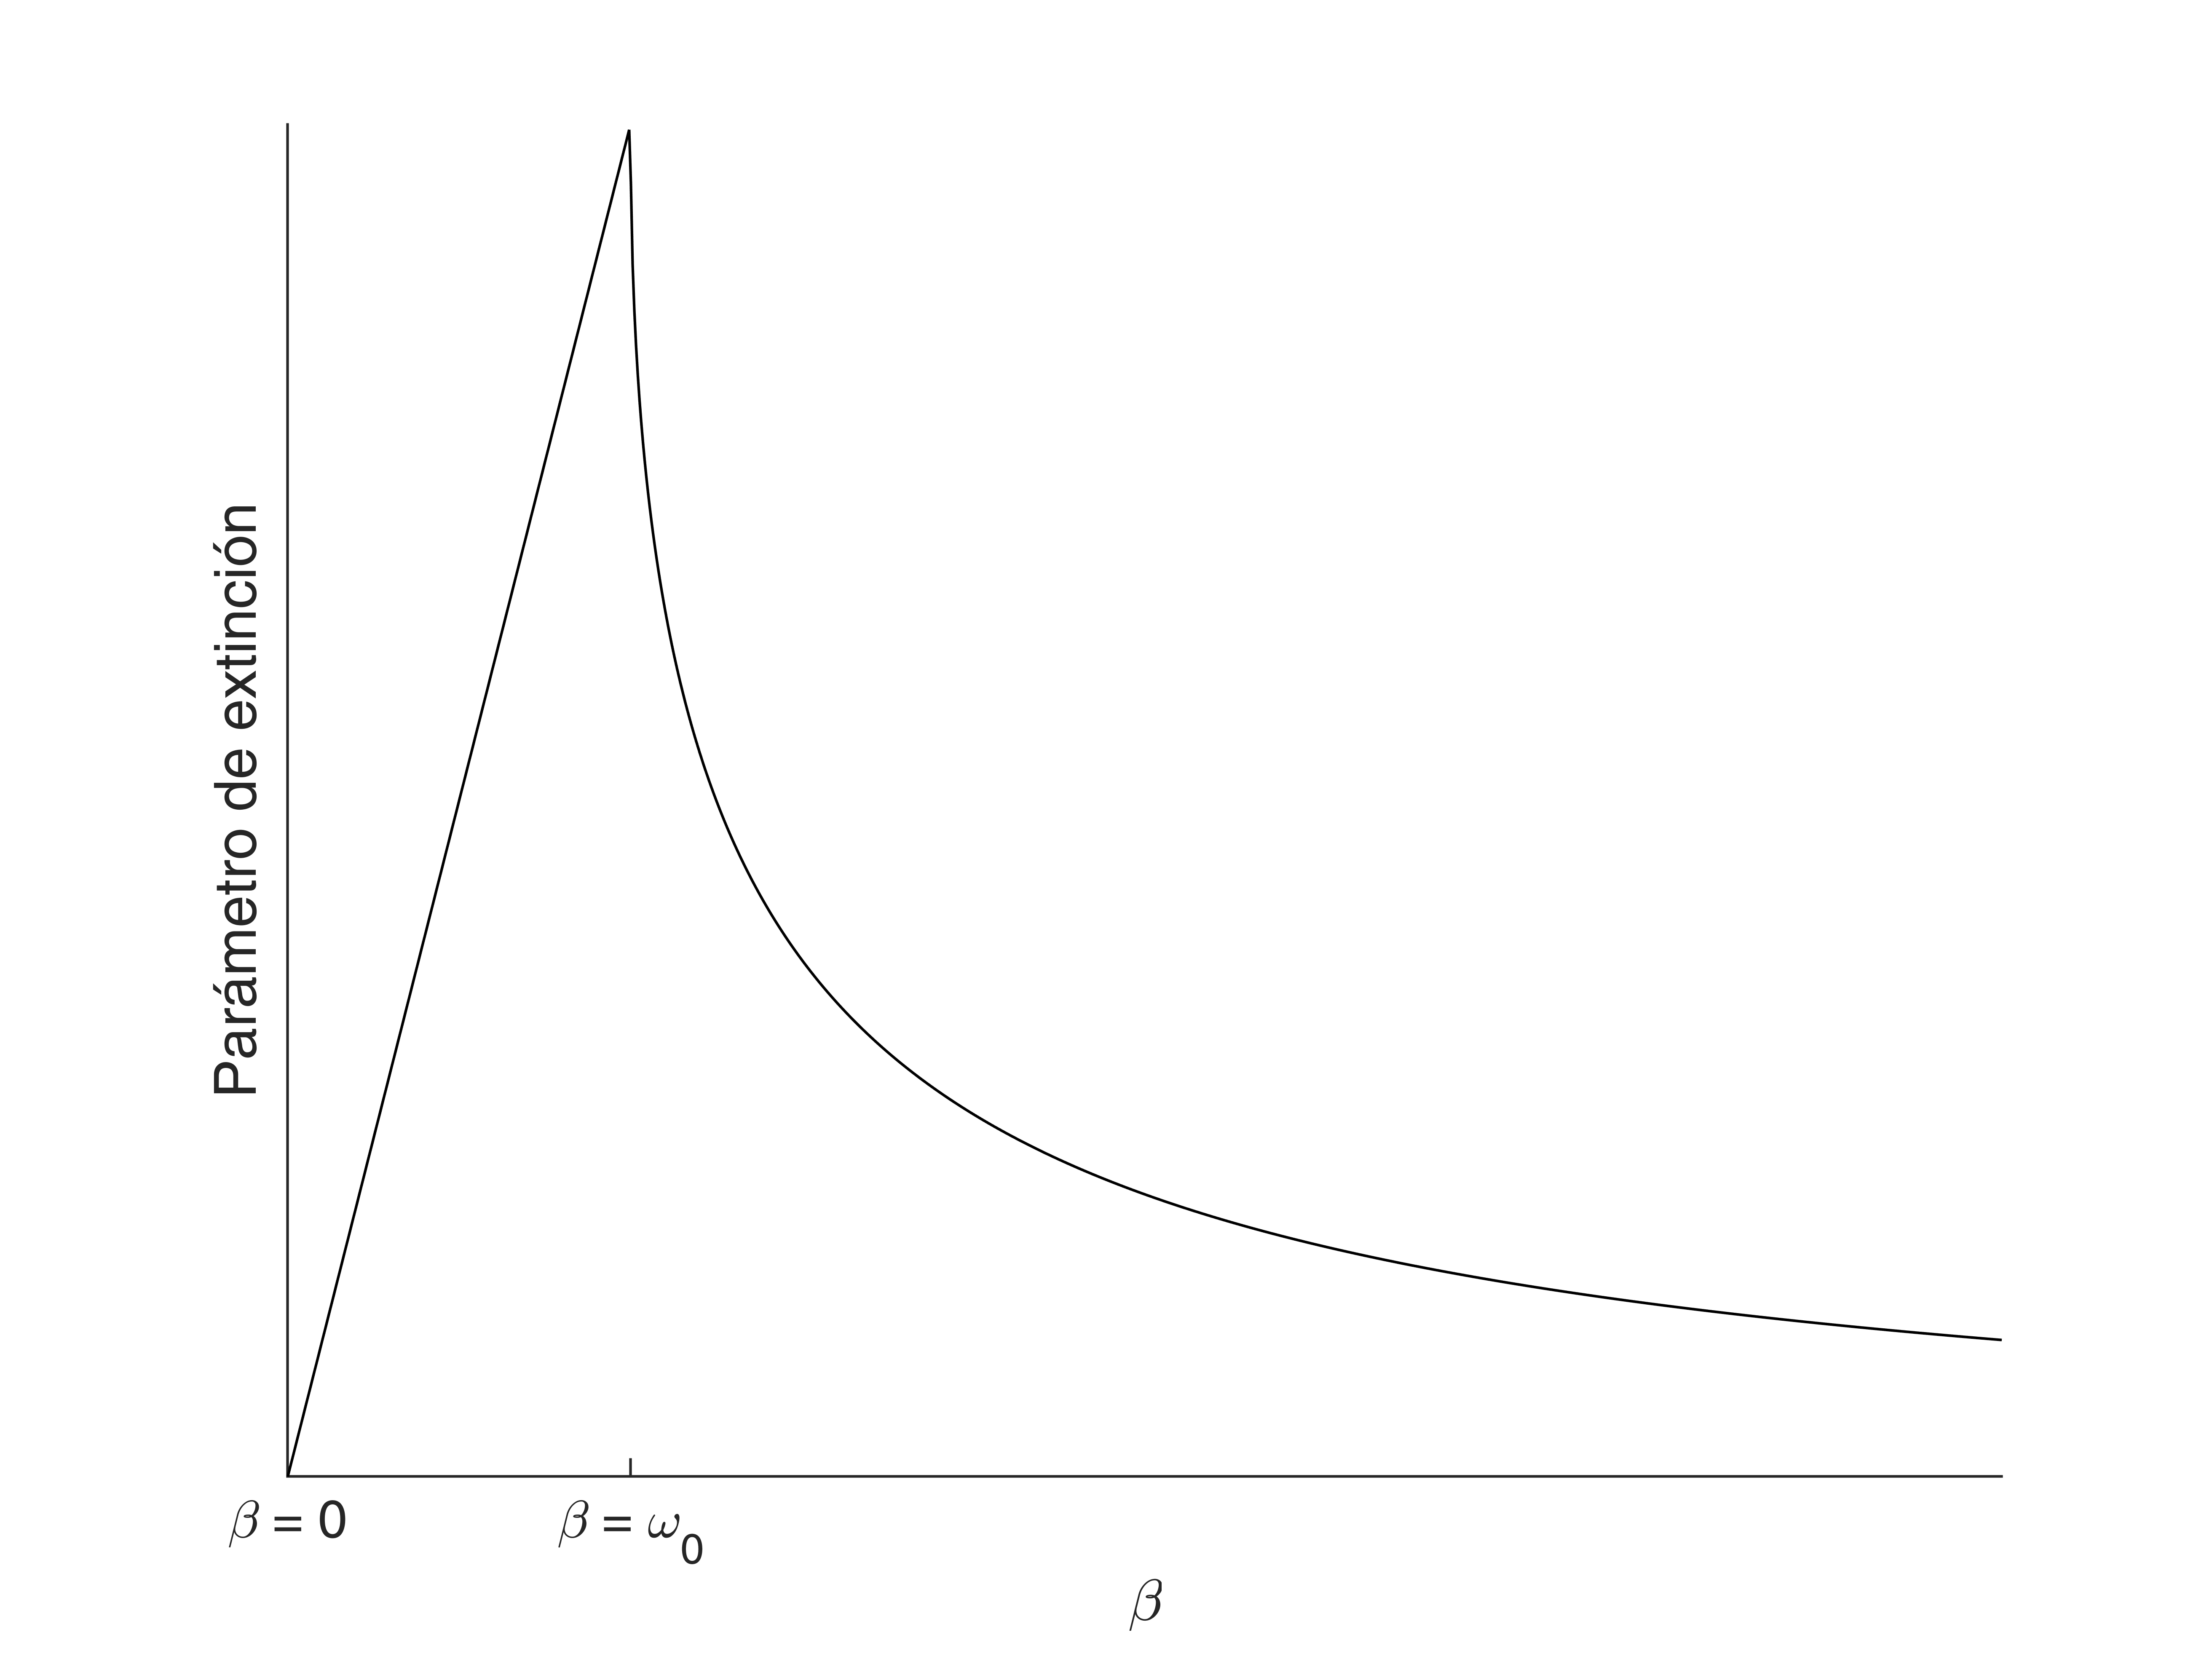
\includegraphics[width=4cm]{images/extin.png}
\end{tikzpicture}
De tal forma que como $a_2 > a_1$ el primer término es el que primará a tiempos largos y por lo tanto el parámetro de extinción será $a_1$.

En este caso ya no tenemos oscilaciones sinusoidales, y en función de las condiciones iniciales, como por ejemplo una velocidad inicial en la posición de equilibrio, tendremos que solo realiza una oscilación, es decir llega a una distancia máxima y a partir de ahí vuelve a la posición de equilibrio sin oscilar más.
\vspace{-15pt}
\subsection{Amortiguamiento crítico}

En el caso en el que $\beta = \omega_0$ tendremos que $\alpha = -\beta$, por lo que como segunda solución linealmente independiente propondremos $te^{\alpha t}$, entonces las ssoluciones nos quedan
\begin{equation} \label{6.1.1}
    x(t) = C_1 e^{-\beta t}(1+C_2t)
\end{equation}\refstepcounter{subsection}
Y de nuevo $\beta$ es el parámetro de extinción.

Si representamos el parámetro de extinción en función de $\beta$ utilizando las expresiones que hemos ido hallando, observamos que la mayor amortiguación ocurre cuando $\beta = \omega_0$, por eso se llama amortiguamiento crítico.

A mayores $\beta$, hay menos posibilidad de amortiguamiento porque el sistema casi no oscila y por lo tanto la velocidad va a ser pequeña.

\refstepcounter{section}
\section{Oscilaciones forzadas}
\refstepcounter{subsection}
Supongamos que tenemos una fuerza externa además de la fuerza elástica y el rozamiento, de tal forma que obtenemos la siguiente ecuación diferencial
\begin{equation} \label{6.1.1}
    \ddot{x} + 2\beta\dot{x} + \omega_0^2 x = f(t) \ \ \ \ \ 2\beta = \frac{b}{m} \ \ \ \ \ \omega_0^2 = \frac{k}{m}  \ \ \ \ \ \ f(t) = \frac{F}{m}
\end{equation}\refstepcounter{subsection}
La solución general será entonces la solución de la parte homogénea, es decir, el oscilador no amortiguado, más la suma de una solución particular de la inhomogénea, puesto que la ecuación es lineal.

Vamos a estudiar el caso concreto de una fuerza de la forma $f(t) = f_0 \cos \omega t$, y para obtener la solución particular, vamos a resolver el caso en el que $f(t) = f_0 e^{i\omega t}$ y tomaremos la parte real de la solución. Esto esta justificado porque la ecuación es lineal y la parte imaginaria de la solución corresponderá a la parte imaginaria del término inhomogéneo.

Entonces para resolver el caso complejo, hacemos la conjetura $\tilde{x}(t) = C e^{i\omega t}$, donde $C \in \mathbb{C}$, de tal forma que nos queda
\begin{equation} \label{6.1.1}
    C(-\omega^2 + 2 i \omega\beta + \omega_0^2 ) e^{i\omega t} = f_0 e^{i\omega t} \implies C = \frac{f_0}{\omega_0^2 -\omega^2 + 2 i \omega\beta}
\end{equation}\refstepcounter{subsection}
Que nos gustaría expresar como $C = A e^{-\delta i}$ en forma polar, para ello calculamos su módulo, tal que
\begin{equation} \label{6.1.1}
    A^2 = C C^* \rightarrow A = \frac{f_0}{\sqrt{\left(\omega_0^2 -\omega^2\right)^2+4\omega^2 \beta^2}}
\end{equation}\refstepcounter{subsection}
Donde el conjugado de una función holomórfica como es el cociente de dos números complejos es simplemente sustituir $i$ por $-i$. Para obtener la fase, queremos expresar $C = a+bi$, de tal forma que $\tan -\delta = b/a$.
\[
    C = \frac{f_0}{\omega_0^2 -\omega^2 + 2 i \omega\beta} \frac{\omega_0^2 -\omega^2 - 2 i \omega\beta}{\omega_0^2 -\omega^2 - 2 i \omega\beta} = K \left[(\omega_0^2 -\omega^2) - i (2\omega\beta)\right] \ \ \ \ \ K \in \mathbb{R}
\]
\begin{equation} \label{6.1.1}
    \tan -\delta = -\frac{2\omega \beta}{\omega_0^2 - \omega^2} \implies \tan \delta = \frac{2\omega \beta}{\omega_0^2 - \omega^2}
\end{equation}\refstepcounter{subsection}
De tal forma que tenemos la solución partícular de la inhomogénea
\begin{equation} \label{6.1.1}
    \tilde{x}(t) = A e^{(\omega t -\delta)i} \implies x(t) = \mathfrak{Re}\{\tilde{x}(t)\}= A \cos(\omega t -\delta)
\end{equation}\refstepcounter{subsection}
Así, la solución general (salvo $\beta=\omega_0$) es 
\begin{equation} \label{6.1.1}
    x(t) = A \cos(\omega t -\delta) + e^{-\beta t} \left(c_1 e^{t\sqrt{\beta^2-\omega_0^2}}+ c_2 e^{-t\sqrt{\beta^2-\omega_0^2}}\right)
\end{equation}\refstepcounter{subsection}
Se observa que el primer término no depende de las condiciones iniciales, y solo de $\omega$, $f_0$, $\omega_0$ y $\beta$, por eso denomina término estacionario.

El segundo sí que depende de las condiciones iniciales, pero el factor $e^{-\beta t}$ hace que este sea muy poco relevante a medida que avanza el tiempo, por eso se denomina término transitorio.
\subsection{Resonancia}
El máximo de $A$ se llama resonancia, para encontrarlo buscaremos el máximo de $A^2$, que es el mismo, y para ello, como el numerador es constante, buscaremos el mínimo del denominador.

Si tomamos $\omega$ fijo y variamos $\omega_0$, tenemos que
\begin{equation} \label{6.1.1}
    \frac{d}{d \omega_0} \left(\left(\omega_0^2 -\omega^2\right)^2+4\omega^2 \beta^2\right) = 4\left(\omega_0^2 -\omega^2\right) \omega_0 = 0   \rightarrow \bar{\omega}_0 = 0 \ \ \ \ \bar{\omega}_0 = \omega
\end{equation}\refstepcounter{subsection}
\[
    \frac{d^2}{d \omega_0^2} \left(\left(\omega_0^2 -\omega^2\right)^2+4\omega^2 \beta^2\right) = 4\left(\omega_0^2 -\omega^2\right) + 8\omega_0^2
\]
\begin{equation} \label{6.1.1}
    \left.\frac{d^2}{d \omega_0^2}\right|_\omega = 8\omega_0^2 > 0 \rightarrow \bar{\omega}_0 = \omega \mbox{ : max. de A} \ \ \ \ \ \left.\frac{d^2}{d \omega_0^2}\right|_0 = -4\omega^2 < 0 \rightarrow  \bar{\omega}_0 = 0 \mbox{ : min. de A} 
\end{equation}\refstepcounter{subsection}

De esta forma, tenemos que la frecuencia de resonancia es $\bar{\omega}_0 = \omega$ y la amplitud máxima es
\begin{equation} \label{6.1.1}
    A_{\mbox{\small max.}} = \frac{f_0}{2\omega \beta}
\end{equation}\refstepcounter{subsection}

Si ahora tomamos $\omega_0$ y variamos $\omega$, tenemos que
\begin{equation} \label{6.1.1}
    \frac{d}{d \omega} \left(\left(\omega_0^2 -\omega^2\right)^2+4\omega^2 \beta^2\right) =\left[8\beta^2-4\left(\omega_0^2 -\omega^2\right)\right]\omega = 0   \rightarrow \bar{\omega} = 0 \ \ \ \ \bar{\omega} =  \sqrt{\omega_0^2-2\beta^2}
\end{equation}\refstepcounter{subsection}
\[
    \frac{d^2}{d \omega^2} \left(\left(\omega_0^2 -\omega^2\right)^2+4\omega^2 \beta^2\right) = \left[8\beta^2-4\left(\omega_0^2 -\omega^2\right)\right] + 8\omega^2
\]
\begin{equation} \label{6.1.1}
    \left.\frac{d^2}{d \omega^2}\right|_0 = 8\beta^2 - 4\omega_0^2  \ \ \ \ \ \left.\frac{d^2}{d \omega^2}\right|_{\sqrt{\omega_0^2-2\beta^2}} = 8\omega_0^2-16\beta^2
\end{equation}\refstepcounter{subsection}
\begin{tikzpicture}[]
    \node [shift={(-16.5cm, -27.8cm)}] at (current page.north east){};
        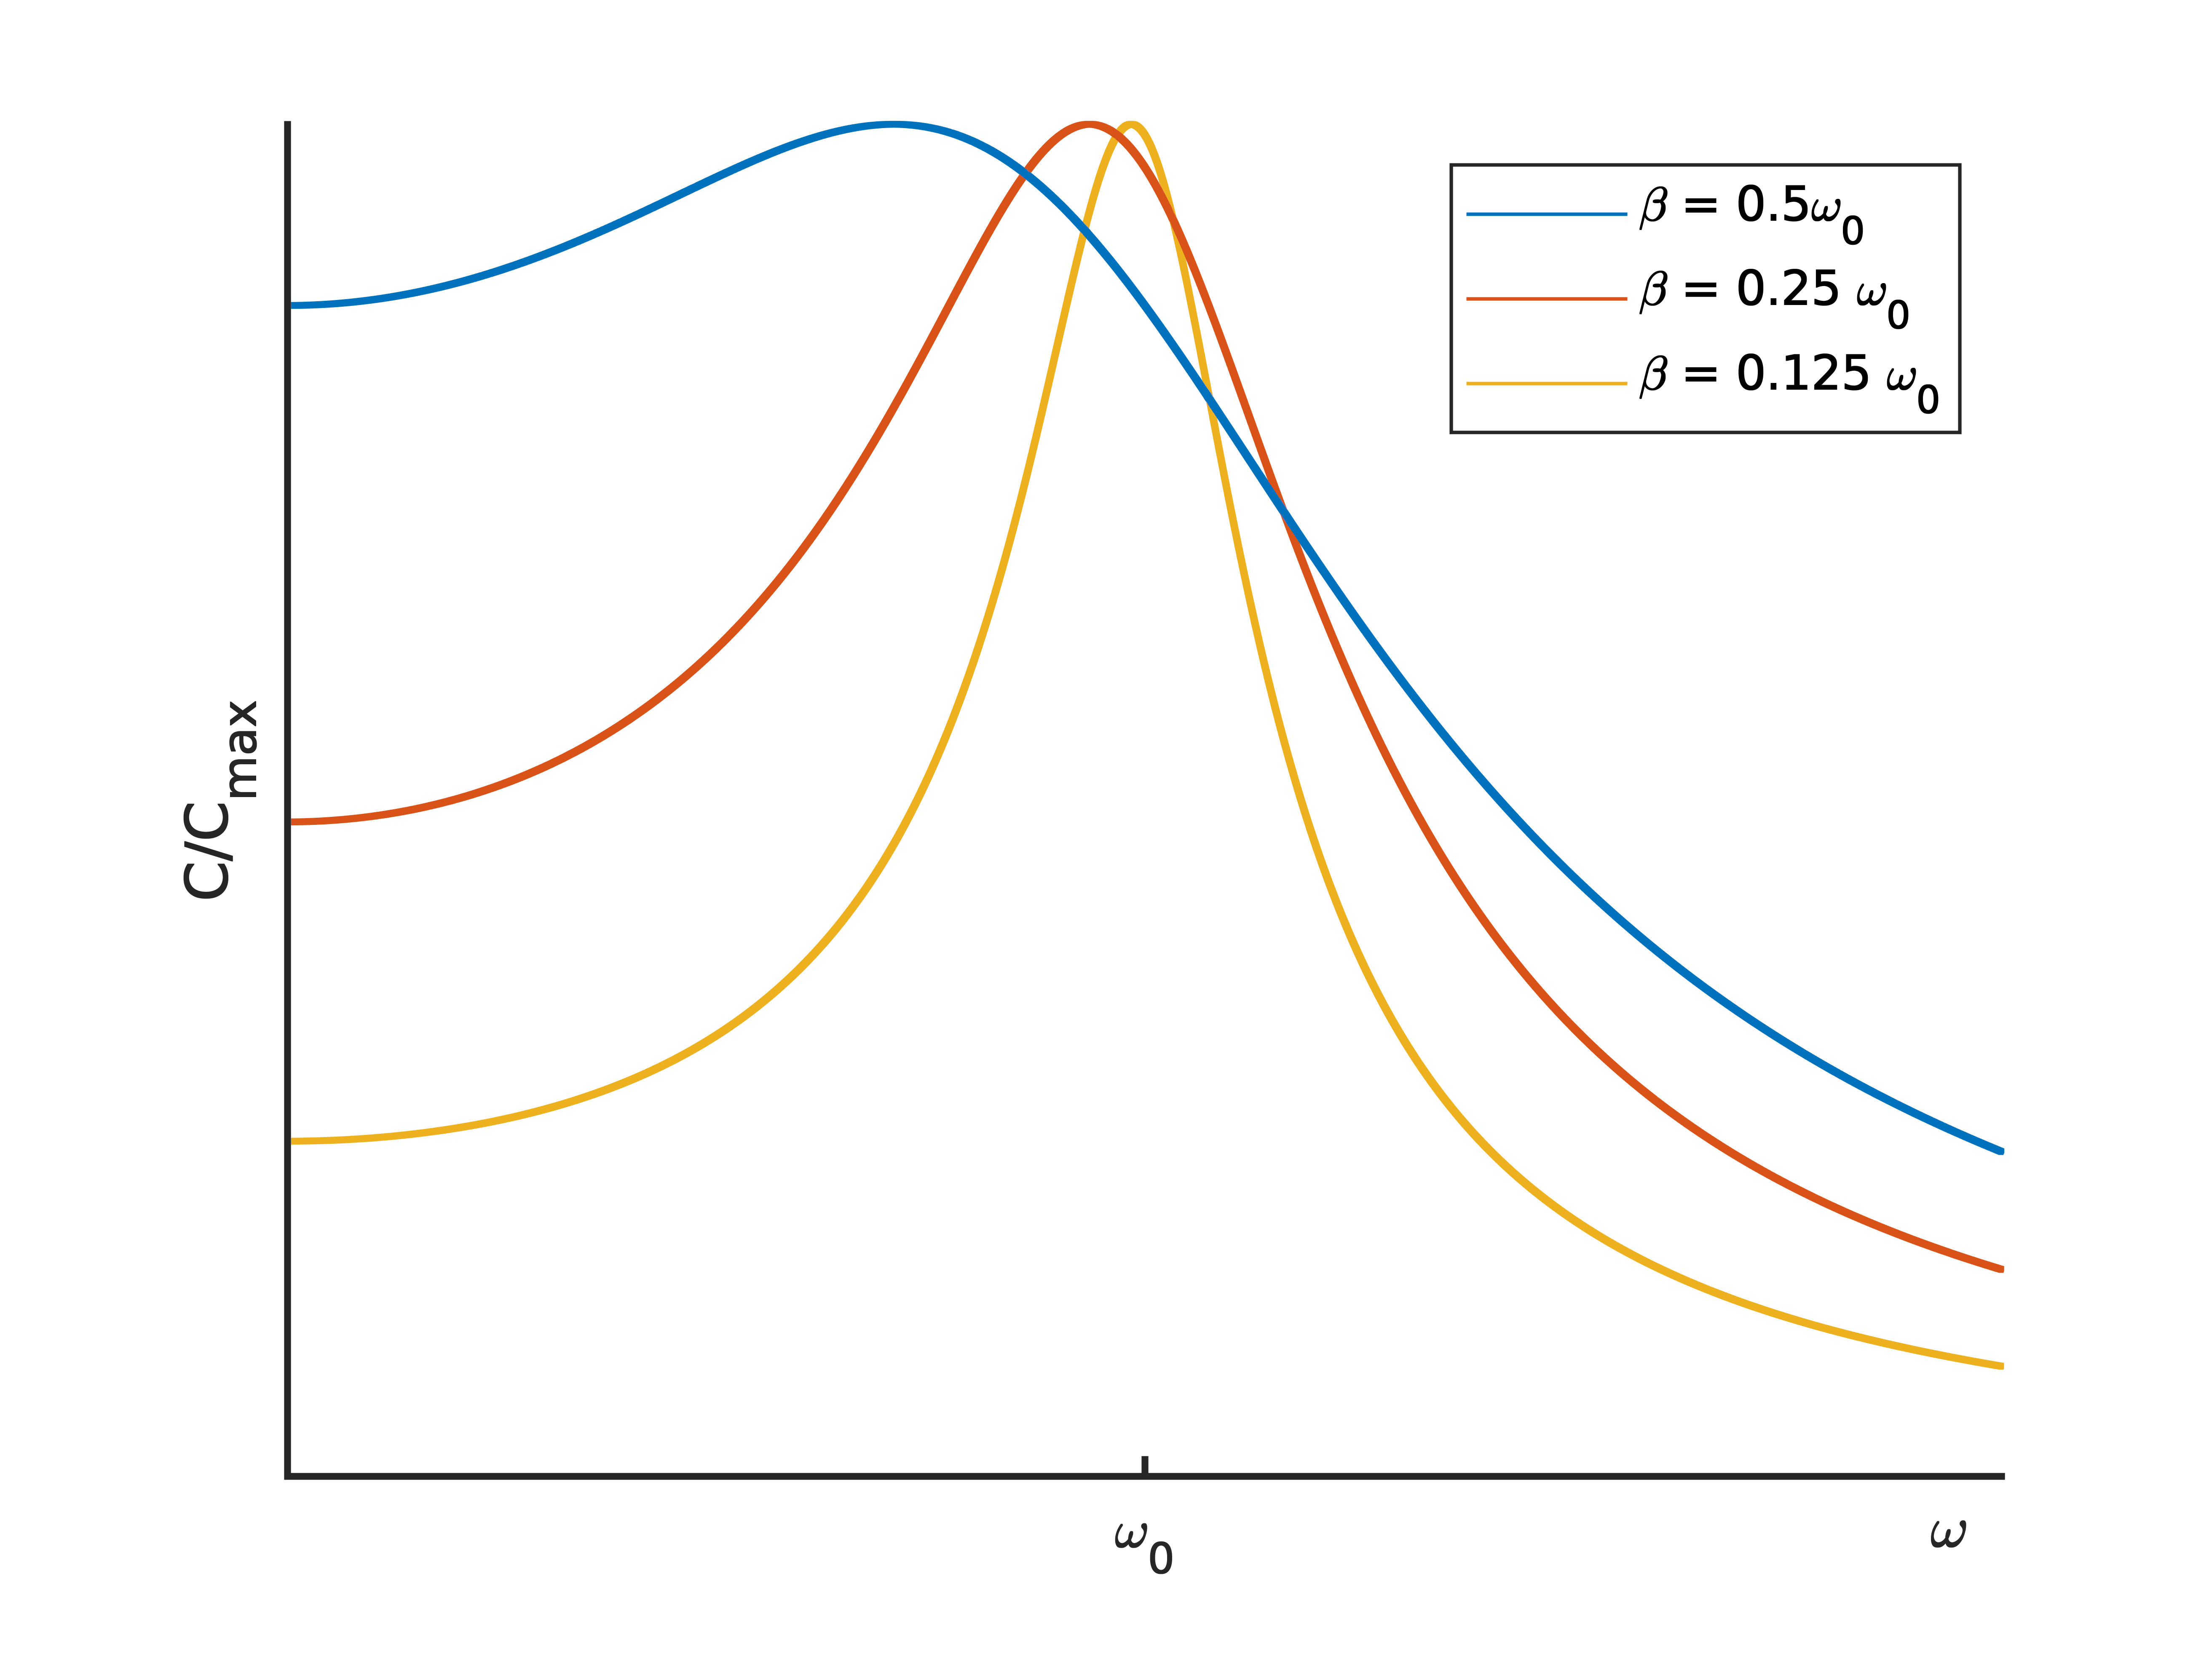
\includegraphics[width=6.3cm]{images/osforz.png}
\end{tikzpicture}
Cuando $\beta > \omega_0 /\sqrt{2}$, tenemos un solo máximo en $\bar{\omega} = 0$.
\begin{equation} \label{6.1.1}
    A_{\mbox{\small max.}} = \frac{f_0}{2\beta \sqrt{\omega_0^2-\beta^2}}
\end{equation}\refstepcounter{subsection}

Si $\beta \ll \omega_0$ (subamortiguado), tenemos que $\bar{\omega} = 0$ es un mínimo de $A$ y $\bar{\omega} = \sqrt{\omega_0^2-2\beta^2} \approx \omega_0$ es un máximo de $A$. El valor de la amplitud máxima para este último es entonces

En la figura lateral se observa la amplitud normalizada en función de  $\omega$ y de distintos valores de $\beta$, y comprobamos que cuando $\beta \ll \omega_0$, $\bar{\omega} \rightarrow \omega_0$, pero en general no es así, y el máximo esta desplazado con respecto a $\omega_0$.
Además, no se observa en la figura, pero sí en la expresión (8.3.11), cuando $\beta \rightarrow 0$, $A_{\mbox{\small max.}} \rightarrow \infty$.
\newpage
\subsubsection{Factor de calidad}
Definimos el factor de calidad como
\begin{equation} \label{6.1.1}
    Q \equiv  \frac{\bar{\omega}}{\Delta \omega}
\end{equation}\refstepcounter{subsection}

\vspace{-15pt}
Dónde $\Delta \omega$ es la anchura a altura media (FWHM por sus siglas en inglés).

Se define originalmente para un oscilador no forzado como el periodo caracterísitico de amortiguamiento de la energía $\beta^{-1}/2$ ($E \propto x^2$) entre el tiempo necesario para oscilar un radian
\begin{equation} \label{6.1.1}
    Q = \frac{\tau / 2}{T/ 2\pi} = \frac{\beta^{-1}/2}{1/\omega} = \frac{\omega}{2\beta} \rightarrow E (t = T) = E_0 e^{-2 \beta (2\pi/\omega)} = E_0 e^{-2\pi/Q}
\end{equation}\refstepcounter{subsection}
\begin{tikzpicture}[remember picture,overlay]
    \node [shift={(-4cm, -8.5cm)}] at (current page.north east)
    {\def\svgwidth{5 cm}
    \input{images/FWHM.pdf_tex}};
\end{tikzpicture}
$Q$ entonces representa el inverso del factor de extinción de la energía \newline por radián. Para sistemas forzados tenemos que es la energía del sistema \newline entre  la energía disipada por radián, y nos queda la misma expresión.

Tenemos además como hemos visto en (8.3.13), se define de forma más general \newline como la frecuencia de resonancia entre la anchura a altura media, que como se observa en la figura, es la anchura de la gráfica $A^2$, en función de $\omega$ cuando 
\begin{equation} \label{6.1.1}
    A(\tilde{\omega})^2 = \frac{A^2_{\mbox{\small max.}}}{2}
\end{equation}\refstepcounter{subsection}
Resolviendo la ecuación de segundo grado en $\tilde{\omega}$ que nos queda y luego haciendo expansiones considerando el caso $\beta \ll \omega_0$ obtenemos el resultado
\begin{equation} \label{6.1.1}
    \tilde{\omega} \approx \omega_0 \pm \beta \implies \Delta \omega \approx 2\beta \implies Q \approx \frac{\omega_0}{2\beta}
\end{equation}\refstepcounter{subsection}
De esta forma $Q$ es una especie de inverso de un error relativo, y cuanto mayor sea este, más estrecha será la banda de resonancia. A su vez, según las interpretaciones anteriores, a mayor $Q$, menor será el amortiguamiento y menor energía será disipada.
\vspace{-15pt}
\subsubsection{Desfase}
\begin{tikzpicture}[]
    \node [shift={(-32cm, -22.5cm)}] at (current page.north east){};
        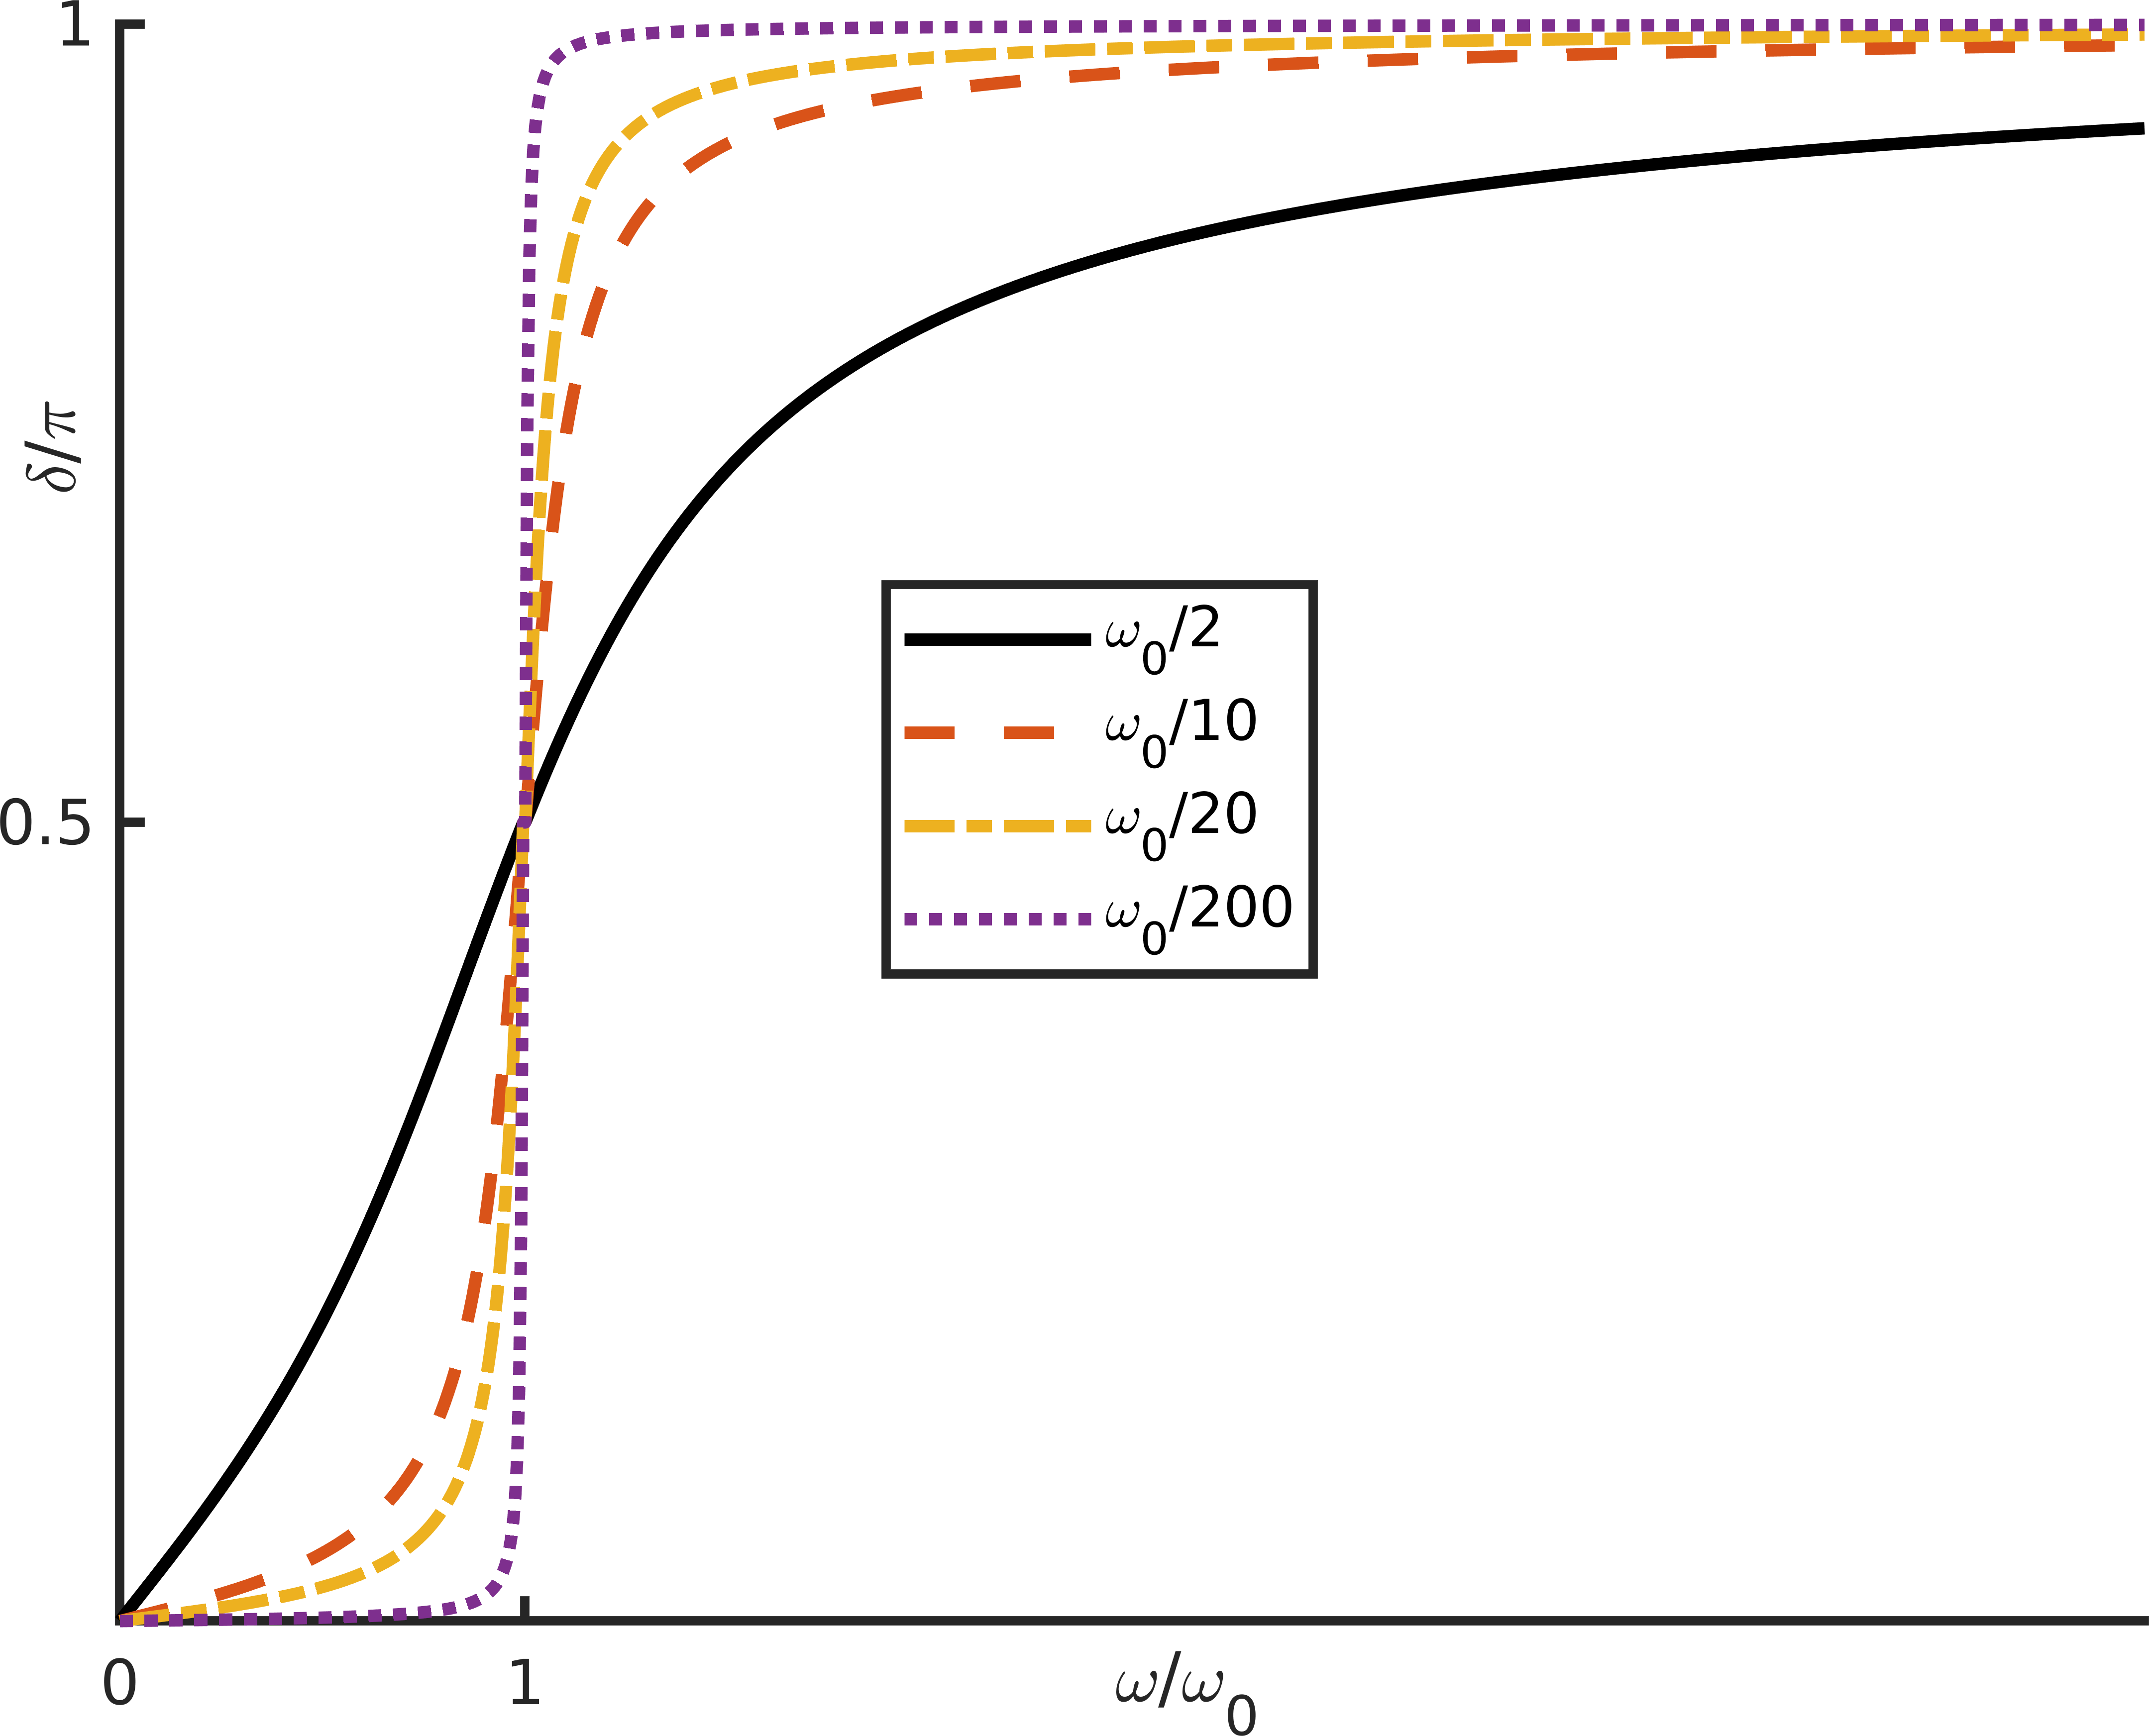
\includegraphics[width=6.3cm]{images/delta.png}
\end{tikzpicture}
Analizando (8.3.4), vemos que cuando $\omega \rightarrow \omega_0$, $\tan \delta \rightarrow \infty$ y por lo tanto $\delta \rightarrow \pi/2 +\pi k_1$. Si $\omega \rightarrow 0^+$, entonces $\tan \delta \rightarrow 0^+$ y $\delta \rightarrow 0 +\pi k_2$, y si $\omega \rightarrow \infty$, entonces $\tan \delta \rightarrow 0^-$ y $\delta \rightarrow 0 +\pi k_3$.

Para que la función sea contínua, tomamos $k=0$ cuando $\omega < \omega_0$ y $k=1$ cuando $\omega > \omega_0$, de tal forma que definimos naturalmente $\delta(\omega_0) = \pi/2$.

Se observa este comportamiento en la figura de la derecha y como \newline cambia la función en términos de $\beta$, haciéndose casi un escalon, \newline pues cuando $\beta \rightarrow 0$, $\tan \delta \rightarrow 0$ y $\delta \rightarrow 0+\pi k$.
\vspace{-15pt}
\subsection{Potencia}
Definimos la potencia en general como la derivada del trabajo \newline producido por una fuerza con respecto al tiempo, que podemos \newline reescribir tal que
\begin{equation} \label{6.1.1}
    P(t) = \frac{dW}{dt} = F \frac{dx}{dt} = F \dot{x} \implies P(t) = \mathbf{F} \cdot \dot{\mathbf{x}}
\end{equation}\refstepcounter{subsection}
Definimos entonces la potencia media como la integral del valor medio de la función $P(t)$ durante un periodo entero, tal que 
\begin{equation} \label{6.1.1}
    \bar{P} = \frac{1}{T} \int_0^T P(t)dt = \frac{1}{T} \int_{-T/2}^{T/2} P(t)dt
\end{equation}\refstepcounter{subsection}
Y haciendo la integral para un oscilador forzado obtenemos el siguiente resutado
\begin{equation} \label{6.1.1}
    P(t)= -m f_0 A \omega \cos(\omega t) \sin(\omega t -\delta) \ \ \ \ \ \bar{P} = \frac{1}{2} m f_0 \omega A \sin\delta 
\end{equation}\refstepcounter{subsection}
\vspace{-30pt}
\refstepcounter{section}
\section{Fourier}\refstepcounter{subsection}
\subsection{Teorema de Fourier}
Sea $f(t)$ una función periódica, es decir, $\exists \ T$ tal que $f(t+T) = f(t) \ \forall \ t$, entoces podemos expresar $f(t)$ de la siguiente forma
\begin{equation} \label{6.1.1}
    f(t) = \sum_{n=0}^\infty a_n \cos (n\omega t) + b_n \sin (n\omega t) \ \ \ \ \ \omega = \frac{2\pi}{T}
\end{equation}\refstepcounter{subsection}
Donde los coeficientes $a_n$ y $b_n$ vienen determinados por 
\begin{equation} \label{6.1.1}
    a_0 = \frac{1}{T}\int_{-\frac{T}{2}}^{\frac{T}{2}} f(t)dt \ \ \ \ \ a_n = \frac{2}{T}\int_{-\frac{T}{2}}^{\frac{T}{2}} f(t)\cos(n\omega t)dt \ \ \ \ \ b_n = \frac{2}{T}\int_{-\frac{T}{2}}^{\frac{T}{2}} f(t)\sin(n\omega t)dt
\end{equation}\refstepcounter{subsection}
Si $f(t)$ es par, $b_n =0 \ \forall \ n$, y si $f(t)$ es impar $a_n =0 \ \forall \ n$.
\subsection{Ortogonalidad}
No se va a demostrar el Teorema de Fourier, eso implicaria demostrar que el conjunto de funciones
\begin{equation} \label{6.1.1}
    \left\{\cos(n\omega t),\sin(n\omega t)\right\} \ \ \forall \ n \in \mathbb{N}_0
\end{equation}\refstepcounter{subsection}
es completo (base de un espacio de Hilbert) y puede generar cualquier función periódica, pero sí podemos demostrar que el conjunto (8.4.3) forman un conjunto ortogonal bajo una determinada forma bilineal simétrica, que definimos como
\begin{equation} \label{6.1.1}
    \langle f,g \rangle = \frac{2}{T}\int_{-\frac{T}{2}}^{\frac{T}{2}} f(t) g(t) dx
\end{equation}\refstepcounter{subsection}
De tal forma que si $\varphi_i$ y $\varphi_j$ son elementos cualesquiera de (8.4.3), se verifica haciendo las integrales correspondientes que 
\begin{equation} \label{6.1.1}
    \langle \varphi_i, \varphi_j \rangle = \delta_{ij}
\end{equation}\refstepcounter{subsection}
Entonces si suponemos que $f(t) = \sum c_k \varphi_k$, como tenemos en (8.4.1), podemos hallar los coeficientes del la siguiente forma
\begin{equation} \label{6.1.1}
    \langle f(t), \varphi_j \rangle =\langle \sum c_k \varphi_k, \varphi_j \rangle =  \sum c_k \langle \varphi_k, \varphi_j \rangle= \sum c_k \delta_{kj} = c_j
\end{equation}\refstepcounter{subsection}
Realmente el sistema no es ortonormal, sino ortogonal, porque $\langle 1,1\rangle = 2$, de ahí que $a_0$ en (8.4.2) sea distinto que $a_n$, pero para $n\geq 1$, si que son ortonormales las funciones de acuerdo con (8.4.4).
\subsection{Teorema de convergencia}
Sea $f(t)$ una función periódica, discontínua en un número numerable de puntos, la expresion (8.4.1) converge a $f(t)$ en los puntos en los que la función es contínua y converge a $[f(t_0^+) + f(t_0^-)]/2$ en los puntos $t_0$ dónde $f(t)$ no es contínua.

Por ejemplo, la función de dientes de sierra, o unos pulsos binarios periódicos, pueden representarse mediante una Serie de Fourier a pesar de no ser contínuas.
\subsection{Oscilador forzado}
Supongamos ahora un oscilador sometido a una fuerza externa genérica $F(t)$ periódica con fracuencia angular $\omega$, de tal forma que la expresión (8.3.1) podemos expresarla usando (8.4.1) como
\begin{equation} \label{6.1.1}
    \ddot{x} +2\beta \dot{x} +\omega_0^2 x = f(t) = \sum_{n=0}^\infty a_n \cos (n\omega t) + b_n \sin (n\omega t)
\end{equation}\refstepcounter{subsection}
Primero tenemos que $x = \sum x_n$, puesto que la ecuación es lineal, y luego que $x_n = \mathfrak{Re}\{Ce^{in\omega t}\}+\mathfrak{Im}\{De^{in\omega t}\}$, de tal forma que 
\begin{equation} \label{6.1.1}
    C(-n^2\omega^2 +2 i\beta n\omega +\omega_0^2)e^{in\omega t} = a_n e^{in\omega t}
\end{equation}\refstepcounter{subsection}
\vspace{-20pt}
\begin{equation} \label{6.1.1}
    D(-n^2\omega^2 +2 i\beta n\omega +\omega_0^2)e^{in\omega t} = b_n e^{in\omega t}
\end{equation}\refstepcounter{subsection}
Nos quedan entonces de forma simlar a (8.3.3), (8.3.4) y (8.3.5), que la solución estacionaria es 
\begin{equation} \label{6.1.1}
    A_n = \frac{a_n}{\sqrt{\left(\omega_0^2 -n^2\omega^2\right)^2+4n^2\omega^2 \beta^2}} \ \ \ \ B_n = \frac{b_n}{\sqrt{\left(\omega_0^2 -n^2\omega^2\right)^2+4n^2\omega^2 \beta^2}}
\end{equation}\refstepcounter{subsection}
\begin{equation} \label{6.1.1}
    \tan \delta_n = \frac{2n\omega \beta}{\omega_0^2 - n^2\omega^2}
\end{equation}\refstepcounter{subsection}
\begin{equation} \label{6.1.1}
    x =  \sum_{n=0}^\infty A_n \cos(n\omega t - \delta_n) + B_n\sin(n\omega t - \delta_n)
\end{equation}\refstepcounter{subsection}